\documentclass[english]{article}

% For norske bokstaver
% \usepackage[T1]{fontenc}
\usepackage{babel}
\usepackage[utf8]{inputenc}
\usepackage{parskip} % for litt mellomrom mellom avsnittene
\usepackage{amsmath}
\usepackage{graphicx}
\usepackage{subfig}

\renewcommand{\thesection}{\Roman{section}}
\renewcommand{\thesubsection}{\alph{subsection}}

\title{TDT4171 Artificial Intelligence Methods\\
\Huge Exercise 1}
\author{Stian Hvatum (hvatum)\\MTDT}

\begin{document}
\maketitle
\line(1,0){340} % 120mm is aprox. width of text field
\tableofcontents
\newpage
\section{5-card Poker Hands}
\subsection{Atomic events}
The number of different poker hands available, is the combination of 52 cards,
choosen 5 at a time. \footnote{If we take
the order into account, the number would be \(52 \cdot 51 \cdot 50 \cdot 49 \cdot
48 = 311875200\). }

\({{52}\choose{5}} = 2598960\)

\subsection{The probability of an atomic event}
The probability of each atomic event is equal, given the dealer is fear. This
means the probability of each event is
\(1/2598960 = 0.0000038477\)

\subsection{The probability of special hands}
\subsubsection{The probability of a Royal Straight Flush}
There are four possible different Royal Straight Flush-hands in poker. Since
their probability each are equal to all other possible hands, the probability of
one of them, are \(0.0000038477 \cdot 4 = 0.00015391\)

\subsubsection{The probability of a Three of a Kind}
In order to get Three of a kind, you need to get 3 cards of the same value, and
2 of any other value. First, we need to be given one card of value and color.
Then we need to be delt 2 more of this color, that is
\({{13}\choose{1}}{{4}\choose{3}} = 13 \cdot 4 = 52\). This is the number of
ways we can choose 3 cards of same value from a normal deck of cards. We need to
multiply this with the number of ways we can choose the rest of the other cards,
wich is to choose 2 cards with a different value, both with any color.
\({{12}\choose{2}}{{4}\choose{1}}{{4}\choose{1}} = 66 \cdot 4 \cdot 4 = 1056\)

The mathematical formula for how many different Three of a Kind will then be:
	\({{13}\choose{1}}{{4}\choose{3}} \cdot {{12}\choose{2}}{{4}\choose{1}}^2 =
	52 * 1056 = 54912\)

Since there are 54912 Three of a Kind hands, and 2598960 poker hands total, the
probability for one of these are \(54912 / 2598960 = 0.021128\).

\line(1,0){340}
\section{Bayesian Network Construction}
\centerline{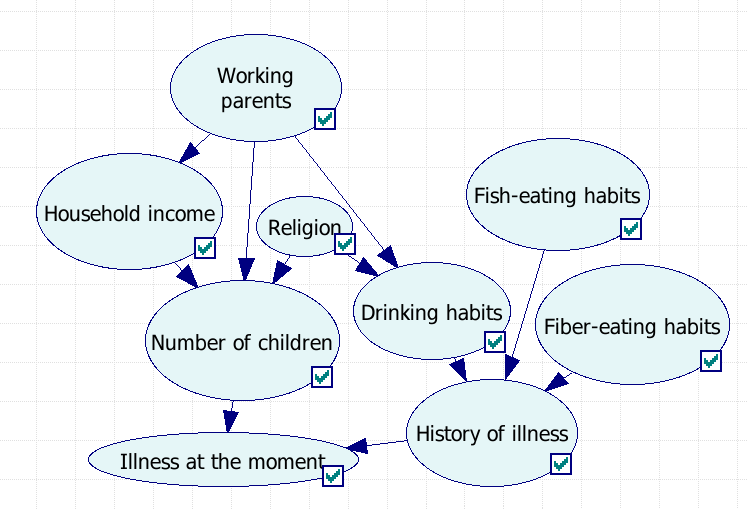
\includegraphics[width=1.4\textwidth]{bay-net-const.png}}
The conditional independence properties of this Bayesian Network are:
\begin{itemize}
  \item Household income, given Working Parents
  \item Number of children, given Household income and Religion
  \item Drinking habits given Working parents and Religion
  \item History of illness given Drinking habits, Fish-eating habits and
  Fiber-eating habits
  \item Illness at the moment given Number of children and History of illness
\end{itemize}
I have chosen Working parents, Fish-eating habits and Fiber-eating habits as the
``independent'' nodes that has no parents.

I would say that in an isolated world, using my knowledge and understanding of
the properties, this assumptions may be perfectly sound. Of course, in the
real world, there are a lot more variables to add to this model. Also, there are
a lot of special cases not well represented in this network.
Eg. if your religion requires you to eat a lot of fiber, there is no doubt that
Fiber-eating habits should have Religion as parent, but in the general case, not
so.

\line(1,0){340}
\newpage
\section{Bayesian Network Application}
I have constructed the Bayesian Network in GeNIe 2.0, and will explain with
screenshots from the analysis of the network I made. The network-file is
attached with the delivery of this exercise and is named
\emph{Bay-net-application.xdsl}.

\begin{figure}[h]
	\subfloat[Initial]{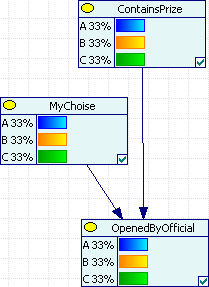
\includegraphics[width=104px]{BNA-1.png}}
	\subfloat[Choise made]{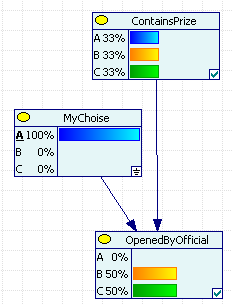
\includegraphics[width=104px]{BNA-2.png}}
	\subfloat[Official opened door]{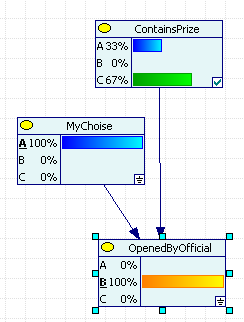
\includegraphics[width=104px]{BNA-3.png}}
	\caption{Flow of events and their effects}
\end{figure}

(a) We see that before we have made any choise, the chance of selecting any of
the doors is \(1/3\) each.

(b) After we have made a choise of wich door we want to open, there no change in
the probability of selecting the right door, still 1/3.

(c) After the official has opened the door, we see that the door we chose, stil
has a probability of 1/3 for containing the prize, while the door left closed by the
official has a probability of 2/3 for containing the prize.

We see here that if we are asked if we want to alter our choise, we should
always answer ``Yes!''. It is easy to think that the probaility is 1/2 for each
of the remaining doors, but we have just seen that this is not the case. 


\end{document}
